% Options for packages loaded elsewhere
\PassOptionsToPackage{unicode}{hyperref}
\PassOptionsToPackage{hyphens}{url}
\PassOptionsToPackage{dvipsnames,svgnames,x11names}{xcolor}
%
\documentclass[
  12pt,
]{article}

\usepackage{amsmath,amssymb}
\usepackage{iftex}
\ifPDFTeX
  \usepackage[T1]{fontenc}
  \usepackage[utf8]{inputenc}
  \usepackage{textcomp} % provide euro and other symbols
\else % if luatex or xetex
  \usepackage{unicode-math}
  \defaultfontfeatures{Scale=MatchLowercase}
  \defaultfontfeatures[\rmfamily]{Ligatures=TeX,Scale=1}
\fi
\usepackage{lmodern}
\ifPDFTeX\else  
    % xetex/luatex font selection
\fi
% Use upquote if available, for straight quotes in verbatim environments
\IfFileExists{upquote.sty}{\usepackage{upquote}}{}
\IfFileExists{microtype.sty}{% use microtype if available
  \usepackage[]{microtype}
  \UseMicrotypeSet[protrusion]{basicmath} % disable protrusion for tt fonts
}{}
\makeatletter
\@ifundefined{KOMAClassName}{% if non-KOMA class
  \IfFileExists{parskip.sty}{%
    \usepackage{parskip}
  }{% else
    \setlength{\parindent}{0pt}
    \setlength{\parskip}{6pt plus 2pt minus 1pt}}
}{% if KOMA class
  \KOMAoptions{parskip=half}}
\makeatother
\usepackage{xcolor}
\usepackage[top=20mm,left=15mm,right=15mm,bottom=20mm]{geometry}
\setlength{\emergencystretch}{3em} % prevent overfull lines
\setcounter{secnumdepth}{5}
% Make \paragraph and \subparagraph free-standing
\ifx\paragraph\undefined\else
  \let\oldparagraph\paragraph
  \renewcommand{\paragraph}[1]{\oldparagraph{#1}\mbox{}}
\fi
\ifx\subparagraph\undefined\else
  \let\oldsubparagraph\subparagraph
  \renewcommand{\subparagraph}[1]{\oldsubparagraph{#1}\mbox{}}
\fi


\providecommand{\tightlist}{%
  \setlength{\itemsep}{0pt}\setlength{\parskip}{0pt}}\usepackage{longtable,booktabs,array}
\usepackage{calc} % for calculating minipage widths
% Correct order of tables after \paragraph or \subparagraph
\usepackage{etoolbox}
\makeatletter
\patchcmd\longtable{\par}{\if@noskipsec\mbox{}\fi\par}{}{}
\makeatother
% Allow footnotes in longtable head/foot
\IfFileExists{footnotehyper.sty}{\usepackage{footnotehyper}}{\usepackage{footnote}}
\makesavenoteenv{longtable}
\usepackage{graphicx}
\makeatletter
\def\maxwidth{\ifdim\Gin@nat@width>\linewidth\linewidth\else\Gin@nat@width\fi}
\def\maxheight{\ifdim\Gin@nat@height>\textheight\textheight\else\Gin@nat@height\fi}
\makeatother
% Scale images if necessary, so that they will not overflow the page
% margins by default, and it is still possible to overwrite the defaults
% using explicit options in \includegraphics[width, height, ...]{}
\setkeys{Gin}{width=\maxwidth,height=\maxheight,keepaspectratio}
% Set default figure placement to htbp
\makeatletter
\def\fps@figure{htbp}
\makeatother

\usepackage{fancyhdr}
\pagestyle{fancy}
\fancyhead[R]{ENSGSI 2AP - Mécanique des Solidés Déformables}

\fancyfoot[L]{Guillaume PRONOST | Fabio CRUZ}
\fancyfoot[C]{\thepage}
\fancyfoot[R]{ENSGSI - 2023/2024}
\renewcommand{\footrulewidth}{0.3pt}% default is 0pt
\setlength{\headheight}{15pt}
\usepackage{mathtools}
\usepackage[makeroom]{cancel}




\makeatletter
\@ifpackageloaded{tcolorbox}{}{\usepackage[skins,breakable]{tcolorbox}}
\@ifpackageloaded{fontawesome5}{}{\usepackage{fontawesome5}}
\definecolor{quarto-callout-color}{HTML}{909090}
\definecolor{quarto-callout-note-color}{HTML}{0758E5}
\definecolor{quarto-callout-important-color}{HTML}{CC1914}
\definecolor{quarto-callout-warning-color}{HTML}{EB9113}
\definecolor{quarto-callout-tip-color}{HTML}{00A047}
\definecolor{quarto-callout-caution-color}{HTML}{FC5300}
\definecolor{quarto-callout-color-frame}{HTML}{acacac}
\definecolor{quarto-callout-note-color-frame}{HTML}{4582ec}
\definecolor{quarto-callout-important-color-frame}{HTML}{d9534f}
\definecolor{quarto-callout-warning-color-frame}{HTML}{f0ad4e}
\definecolor{quarto-callout-tip-color-frame}{HTML}{02b875}
\definecolor{quarto-callout-caution-color-frame}{HTML}{fd7e14}
\makeatother
\makeatletter
\makeatother
\makeatletter
\makeatother
\makeatletter
\@ifpackageloaded{caption}{}{\usepackage{caption}}
\AtBeginDocument{%
\ifdefined\contentsname
  \renewcommand*\contentsname{Table of contents}
\else
  \newcommand\contentsname{Table of contents}
\fi
\ifdefined\listfigurename
  \renewcommand*\listfigurename{List of Figures}
\else
  \newcommand\listfigurename{List of Figures}
\fi
\ifdefined\listtablename
  \renewcommand*\listtablename{List of Tables}
\else
  \newcommand\listtablename{List of Tables}
\fi
\ifdefined\figurename
  \renewcommand*\figurename{Figure}
\else
  \newcommand\figurename{Figure}
\fi
\ifdefined\tablename
  \renewcommand*\tablename{Table}
\else
  \newcommand\tablename{Table}
\fi
}
\@ifpackageloaded{float}{}{\usepackage{float}}
\floatstyle{ruled}
\@ifundefined{c@chapter}{\newfloat{codelisting}{h}{lop}}{\newfloat{codelisting}{h}{lop}[chapter]}
\floatname{codelisting}{Listing}
\newcommand*\listoflistings{\listof{codelisting}{List of Listings}}
\makeatother
\makeatletter
\@ifpackageloaded{caption}{}{\usepackage{caption}}
\@ifpackageloaded{subcaption}{}{\usepackage{subcaption}}
\makeatother
\makeatletter
\@ifpackageloaded{tcolorbox}{}{\usepackage[skins,breakable]{tcolorbox}}
\makeatother
\makeatletter
\@ifundefined{shadecolor}{\definecolor{shadecolor}{rgb}{.97, .97, .97}}
\makeatother
\makeatletter
\makeatother
\makeatletter
\makeatother
\ifLuaTeX
  \usepackage{selnolig}  % disable illegal ligatures
\fi
\IfFileExists{bookmark.sty}{\usepackage{bookmark}}{\usepackage{hyperref}}
\IfFileExists{xurl.sty}{\usepackage{xurl}}{} % add URL line breaks if available
\urlstyle{same} % disable monospaced font for URLs
\hypersetup{
  pdftitle={TD 1: Referentiel de mouvement},
  colorlinks=true,
  linkcolor={blue},
  filecolor={Maroon},
  citecolor={Blue},
  urlcolor={Blue},
  pdfcreator={LaTeX via pandoc}}

\title{TD 1: Referentiel de mouvement}
\usepackage{etoolbox}
\makeatletter
\providecommand{\subtitle}[1]{% add subtitle to \maketitle
  \apptocmd{\@title}{\par {\large #1 \par}}{}{}
}
\makeatother
\subtitle{Objectif: Comprendre les différences entre les notions de
coordonnées de \textbf{base de projection} et de \textbf{référentiel}}
\author{}
\date{}

\begin{document}
\maketitle
\ifdefined\Shaded\renewenvironment{Shaded}{\begin{tcolorbox}[frame hidden, enhanced, interior hidden, borderline west={3pt}{0pt}{shadecolor}, boxrule=0pt, breakable, sharp corners]}{\end{tcolorbox}}\fi

\thispagestyle{fancy}

\hypertarget{exercice-1---base-fixe-base-mobile}{%
\section{Exercice 1 - Base fixe, base
mobile}\label{exercice-1---base-fixe-base-mobile}}

On se place dans un repère en coordonnées cartésiennes
(\(\vec u_x\),\(\vec u_y\)). On place un point \(M\) de coordonnées
(\(x\),\(y\)).

\begin{enumerate}
\def\labelenumi{\arabic{enumi}.}
\item
  Faire un schéma du repère. Placer le point \(M\). Donner l'expression
  du vecteur \(\vec{OM}\), de la vitesse du point \(M\) \(\vec v_M\), et
  de son accélération \(\vec a_M\) dans la base
  (\(\vec u_x\),\(\vec u_y\)) en utilisant les coordonnées cartésiennes
  (\(x\),\(y\)).
\item
  Donner l'expression du vecteur \(\vec{OM}\) dans la base mobile
  (\(\vec u_r\),\(\vec u_\theta\)). Donner l'expression des vecteurs
  \(\vec u_r\) et \(\vec u_\theta\) dans la base
  (\(\vec u_x\),\(\vec u_y\)). Dessiner la base mobile sur votre schéma.
\item
  A l'aide de la question précédente, exprimer les coordonnées
  cartésiennes (\(x\),\(y\)) en fonction des coordonnées polaires
  (\(r\), \(\theta\)). Exprimer \(\vec{OM}\) dans la base fixe
  (\(\vec u_x\),\(\vec u_y\)) en utilisant les coordonnées polaires.
\item
  Exprimer la vitesse du mobile par rapport au référentiel des
  coordonnées cartésiennes \(R_c\), en utilisant les coordonnées
  polaires (\(r\), \(\theta\)) dans la base fixe
  (\(\vec u_x\),\(\vec u_y\)) puis dans la base mobile
  (\(\vec u_r\),\(\vec u_\theta\)). Vérifier qu'il s'agit de la même
  vitesse exprimée sur deux bases différentes.
\end{enumerate}

\hypertarget{solutions}{%
\subsection{Solutions}\label{solutions}}

\hypertarget{question-1-faire-un-schuxe9ma-du-repuxe8re}{%
\subsubsection{Question 1: Faire un schéma du
repère}\label{question-1-faire-un-schuxe9ma-du-repuxe8re}}

On se place dans un repère en coordonnées cartésiennes
(\(\vec u_x\),\(\vec u_y\)). On place un point \(M\) de coordonnées
(\(x\),\(y\)).

\begin{figure}

\begin{minipage}[t]{0.50\linewidth}

{\centering 

\begin{figure}

{\centering 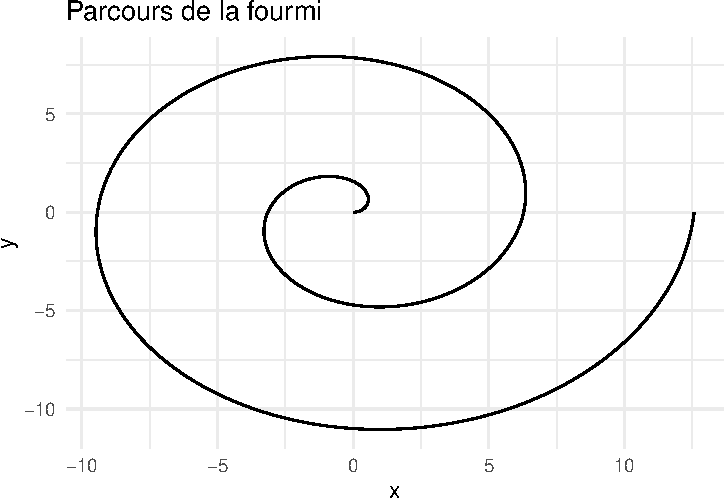
\includegraphics{01-TD_files/figure-pdf/unnamed-chunk-1-1.pdf}

}

\end{figure}

}

\end{minipage}%
%
\begin{minipage}[t]{0.50\linewidth}

{\centering 

}

\end{minipage}%

\end{figure}

\hypertarget{question-2-expression-du-vecteur-vecom}{%
\subsubsection{\texorpdfstring{Question 2: expression du vecteur
\(\vec{OM}\)}{Question 2: expression du vecteur \textbackslash vec\{OM\}}}\label{question-2-expression-du-vecteur-vecom}}

En coordonnées cartésiennes:

\begin{align*}
    \vec{OM} &= x \vec u_x + y \vec u_y\\
    \vec{v(M)} &= \dfrac{dx}{dt} \vec u_x + \dfrac{dy}{dt} \vec u_y\\
    \vec{a(M)} &= \dfrac{d^2x}{dt^2} \vec u_x + \dfrac{d^2y}{dt^2} \vec u_y
\end{align*}

\hypertarget{question-3-expression-du-vecteur-vecom}{%
\subsubsection{\texorpdfstring{Question 3: expression du vecteur
\(\vec{OM}\)}{Question 3: expression du vecteur \textbackslash vec\{OM\}}}\label{question-3-expression-du-vecteur-vecom}}

En coordonnées polaires (\(r\), \(\theta\)):

\begin{align*}
    \vec{OM} &= r \vec u_r \\
    \vec u_r &= \cos{\theta} \vec u_x + \sin{\theta} \vec u_y \ \text{;} \  \vec u_\theta = \sin{\theta} \vec u_x + \cos{\theta} \vec u_y
\end{align*}

\hypertarget{exercise-3-combinaison-mouvement-lineaire-et-mouvement}{%
\section{Exercise 3: Combinaison mouvement lineaire et
mouvement}\label{exercise-3-combinaison-mouvement-lineaire-et-mouvement}}

Il est impératif de bien comprendre qu'on peut exprimer une vitesse
relative à relative à un référentiel. Le mouvement d'un point est donc
relatif à un observateur fixe dans un référentiel d'étude.

\begin{tcolorbox}[enhanced jigsaw, toptitle=1mm, title=\textcolor{quarto-callout-tip-color}{\faLightbulb}\hspace{0.5em}{Tip}, left=2mm, colback=white, breakable, colframe=quarto-callout-tip-color-frame, leftrule=.75mm, bottomrule=.15mm, toprule=.15mm, coltitle=black, bottomtitle=1mm, opacityback=0, titlerule=0mm, arc=.35mm, rightrule=.15mm, opacitybacktitle=0.6, colbacktitle=quarto-callout-tip-color!10!white]

Un \textbf{référentiel} (ou \textbf{solide de référence}) est un
ensemble de points tous fixes les uns par rapport aux autres.
L'observateur qui étudie le mouvement d'un point est lui-même immobile
dans ce référentiel.

\end{tcolorbox}

Si l'on considère une vitesse liée à un référentiel fixe, il faut
comprendre qu'il est parfois plus simple d'exprimer celle-ci sur une
base tournante.

\begin{quote}
Rappel: Un vecteur peut changer dans le termps en ``\emph{tournant}'',
il faut toujours savoir dans quel réferentiel on dérive un vecteur
\end{quote}



\end{document}
